\documentclass[twoside]{book}

% Packages required by doxygen
\usepackage{fixltx2e}
\usepackage{calc}
\usepackage{doxygen}
\usepackage[export]{adjustbox} % also loads graphicx
\usepackage{graphicx}
\usepackage[utf8]{inputenc}
\usepackage{makeidx}
\usepackage{multicol}
\usepackage{multirow}
\PassOptionsToPackage{warn}{textcomp}
\usepackage{textcomp}
\usepackage[nointegrals]{wasysym}
\usepackage[table]{xcolor}

% Font selection
\usepackage[T1]{fontenc}
\usepackage[scaled=.90]{helvet}
\usepackage{courier}
\usepackage{amssymb}
\usepackage{sectsty}
\renewcommand{\familydefault}{\sfdefault}
\allsectionsfont{%
  \fontseries{bc}\selectfont%
  \color{darkgray}%
}
\renewcommand{\DoxyLabelFont}{%
  \fontseries{bc}\selectfont%
  \color{darkgray}%
}
\newcommand{\+}{\discretionary{\mbox{\scriptsize$\hookleftarrow$}}{}{}}

% Page & text layout
\usepackage{geometry}
\geometry{%
  a4paper,%
  top=2.5cm,%
  bottom=2.5cm,%
  left=2.5cm,%
  right=2.5cm%
}
\tolerance=750
\hfuzz=15pt
\hbadness=750
\setlength{\emergencystretch}{15pt}
\setlength{\parindent}{0cm}
\setlength{\parskip}{3ex plus 2ex minus 2ex}
\makeatletter
\renewcommand{\paragraph}{%
  \@startsection{paragraph}{4}{0ex}{-1.0ex}{1.0ex}{%
    \normalfont\normalsize\bfseries\SS@parafont%
  }%
}
\renewcommand{\subparagraph}{%
  \@startsection{subparagraph}{5}{0ex}{-1.0ex}{1.0ex}{%
    \normalfont\normalsize\bfseries\SS@subparafont%
  }%
}
\makeatother

% Headers & footers
\usepackage{fancyhdr}
\pagestyle{fancyplain}
\fancyhead[LE]{\fancyplain{}{\bfseries\thepage}}
\fancyhead[CE]{\fancyplain{}{}}
\fancyhead[RE]{\fancyplain{}{\bfseries\leftmark}}
\fancyhead[LO]{\fancyplain{}{\bfseries\rightmark}}
\fancyhead[CO]{\fancyplain{}{}}
\fancyhead[RO]{\fancyplain{}{\bfseries\thepage}}
\fancyfoot[LE]{\fancyplain{}{}}
\fancyfoot[CE]{\fancyplain{}{}}
\fancyfoot[RE]{\fancyplain{}{\bfseries\scriptsize Generated by Doxygen }}
\fancyfoot[LO]{\fancyplain{}{\bfseries\scriptsize Generated by Doxygen }}
\fancyfoot[CO]{\fancyplain{}{}}
\fancyfoot[RO]{\fancyplain{}{}}
\renewcommand{\footrulewidth}{0.4pt}
\renewcommand{\chaptermark}[1]{%
  \markboth{#1}{}%
}
\renewcommand{\sectionmark}[1]{%
  \markright{\thesection\ #1}%
}

% Indices & bibliography
\usepackage{natbib}
\usepackage[titles]{tocloft}
\setcounter{tocdepth}{3}
\setcounter{secnumdepth}{5}
\makeindex

% Hyperlinks (required, but should be loaded last)
\usepackage{ifpdf}
\ifpdf
  \usepackage[pdftex,pagebackref=true]{hyperref}
\else
  \usepackage[ps2pdf,pagebackref=true]{hyperref}
\fi
\hypersetup{%
  colorlinks=true,%
  linkcolor=blue,%
  citecolor=blue,%
  unicode%
}

% Custom commands
\newcommand{\clearemptydoublepage}{%
  \newpage{\pagestyle{empty}\cleardoublepage}%
}

\usepackage{caption}
\captionsetup{labelsep=space,justification=centering,font={bf},singlelinecheck=off,skip=4pt,position=top}

%===== C O N T E N T S =====

\begin{document}

% Titlepage & ToC
\hypersetup{pageanchor=false,
             bookmarksnumbered=true,
             pdfencoding=unicode
            }
\pagenumbering{roman}
\begin{titlepage}
\vspace*{7cm}
\begin{center}%
{\Large Array\+Bot \\[1ex]\large 0.\+5 }\\
\vspace*{1cm}
{\large Generated by Doxygen 1.8.11}\\
\end{center}
\end{titlepage}
\clearemptydoublepage
\tableofcontents
\clearemptydoublepage
\pagenumbering{arabic}
\hypersetup{pageanchor=true}

%--- Begin generated contents ---
\chapter{Hierarchical Index}
\section{Class Hierarchy}
This inheritance list is sorted roughly, but not completely, alphabetically\+:\begin{DoxyCompactList}
\item \contentsline{section}{A\+B\+Object}{\pageref{class_a_b_object}}{}
\begin{DoxyCompactList}
\item \contentsline{section}{A\+B\+Exception}{\pageref{class_a_b_exception}}{}
\item \contentsline{section}{A\+P\+T\+Device}{\pageref{class_a_p_t_device}}{}
\begin{DoxyCompactList}
\item \contentsline{section}{A\+P\+T\+Motor}{\pageref{class_a_p_t_motor}}{}
\begin{DoxyCompactList}
\item \contentsline{section}{T\+Cube\+D\+C\+Servo}{\pageref{class_t_cube_d_c_servo}}{}
\end{DoxyCompactList}
\end{DoxyCompactList}
\item \contentsline{section}{Device\+Manager}{\pageref{class_device_manager}}{}
\end{DoxyCompactList}
\item exception\begin{DoxyCompactList}
\item \contentsline{section}{A\+B\+Exception}{\pageref{class_a_b_exception}}{}
\end{DoxyCompactList}
\item \contentsline{section}{Scaling\+Factors}{\pageref{struct_scaling_factors}}{}
\item \contentsline{section}{Thor\+Labs\+Data}{\pageref{class_thor_labs_data}}{}
\end{DoxyCompactList}

\chapter{Class Index}
\section{Class List}
Here are the classes, structs, unions and interfaces with brief descriptions\+:\begin{DoxyCompactList}
\item\contentsline{section}{\hyperlink{class_a_b_exception}{A\+B\+Exception} }{\pageref{class_a_b_exception}}{}
\item\contentsline{section}{\hyperlink{class_a_b_object}{A\+B\+Object} }{\pageref{class_a_b_object}}{}
\item\contentsline{section}{\hyperlink{class_a_p_t_device}{A\+P\+T\+Device} }{\pageref{class_a_p_t_device}}{}
\item\contentsline{section}{\hyperlink{class_a_p_t_motor}{A\+P\+T\+Motor} }{\pageref{class_a_p_t_motor}}{}
\item\contentsline{section}{\hyperlink{class_device_manager}{Device\+Manager} }{\pageref{class_device_manager}}{}
\item\contentsline{section}{\hyperlink{struct_scaling_factors}{Scaling\+Factors} }{\pageref{struct_scaling_factors}}{}
\item\contentsline{section}{\hyperlink{class_t_cube_d_c_servo}{T\+Cube\+D\+C\+Servo} }{\pageref{class_t_cube_d_c_servo}}{}
\item\contentsline{section}{\hyperlink{class_thor_labs_data}{Thor\+Labs\+Data} }{\pageref{class_thor_labs_data}}{}
\end{DoxyCompactList}

\chapter{Class Documentation}
\hypertarget{class_a_b_exception}{}\section{A\+B\+Exception Class Reference}
\label{class_a_b_exception}\index{A\+B\+Exception@{A\+B\+Exception}}
Inheritance diagram for A\+B\+Exception\+:\begin{figure}[H]
\begin{center}
\leavevmode
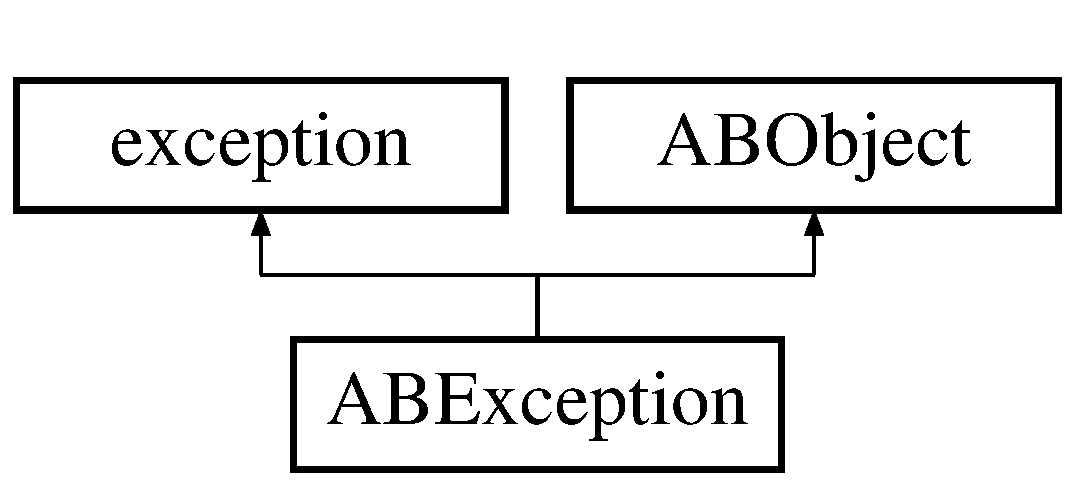
\includegraphics[height=2.000000cm]{class_a_b_exception}
\end{center}
\end{figure}
\subsection*{Public Member Functions}
\begin{DoxyCompactItemize}
\item 
{\bfseries A\+B\+Exception} (const string \&desc)\hypertarget{class_a_b_exception_afe0f40cac5db19bdb8d74da3e1a8433d}{}\label{class_a_b_exception_afe0f40cac5db19bdb8d74da3e1a8433d}

\item 
{\bfseries A\+B\+Exception} (const stringstream \&msg)\hypertarget{class_a_b_exception_a7f702901e7f92811e09583073ede5ba1}{}\label{class_a_b_exception_a7f702901e7f92811e09583073ede5ba1}

\item 
virtual const char $\ast$ {\bfseries what} () const   throw ()\hypertarget{class_a_b_exception_aabde441a97b16beca5b25e203a5f2d40}{}\label{class_a_b_exception_aabde441a97b16beca5b25e203a5f2d40}

\item 
string {\bfseries Message} () const \hypertarget{class_a_b_exception_aa41c1c2b8ba908e5db9c61b5bbc11926}{}\label{class_a_b_exception_aa41c1c2b8ba908e5db9c61b5bbc11926}

\end{DoxyCompactItemize}
\subsection*{Protected Attributes}
\begin{DoxyCompactItemize}
\item 
string {\bfseries m\+Message}\hypertarget{class_a_b_exception_a13d2233110b4ea23196c12c18d6ac593}{}\label{class_a_b_exception_a13d2233110b4ea23196c12c18d6ac593}

\end{DoxyCompactItemize}


\subsection{Detailed Description}


Definition at line 12 of file ab\+Exceptions.\+h.



The documentation for this class was generated from the following files\+:\begin{DoxyCompactItemize}
\item 
source/ab\+Exceptions.\+h\item 
source/ab\+Exceptions.\+cpp\end{DoxyCompactItemize}

\hypertarget{class_a_b_object}{}\section{A\+B\+Object Class Reference}
\label{class_a_b_object}\index{A\+B\+Object@{A\+B\+Object}}
Inheritance diagram for A\+B\+Object\+:\begin{figure}[H]
\begin{center}
\leavevmode
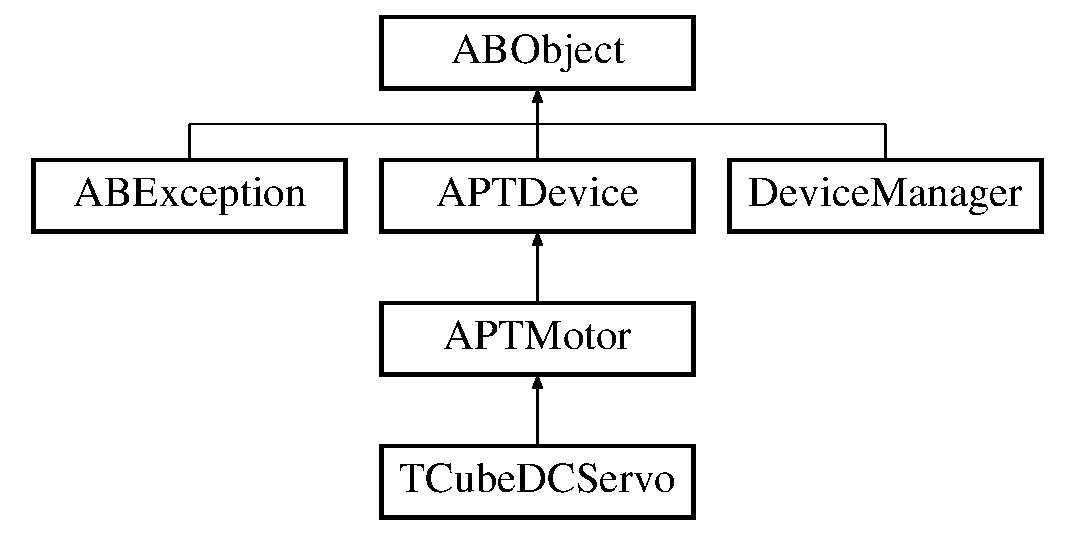
\includegraphics[height=4.000000cm]{class_a_b_object}
\end{center}
\end{figure}


\subsection{Detailed Description}


Definition at line 6 of file ab\+A\+B\+Object.\+h.



The documentation for this class was generated from the following files\+:\begin{DoxyCompactItemize}
\item 
source/ab\+A\+B\+Object.\+h\item 
source/ab\+A\+B\+Object.\+cpp\end{DoxyCompactItemize}

\hypertarget{class_a_p_t_device}{}\section{A\+P\+T\+Device Class Reference}
\label{class_a_p_t_device}\index{A\+P\+T\+Device@{A\+P\+T\+Device}}
Inheritance diagram for A\+P\+T\+Device\+:\begin{figure}[H]
\begin{center}
\leavevmode
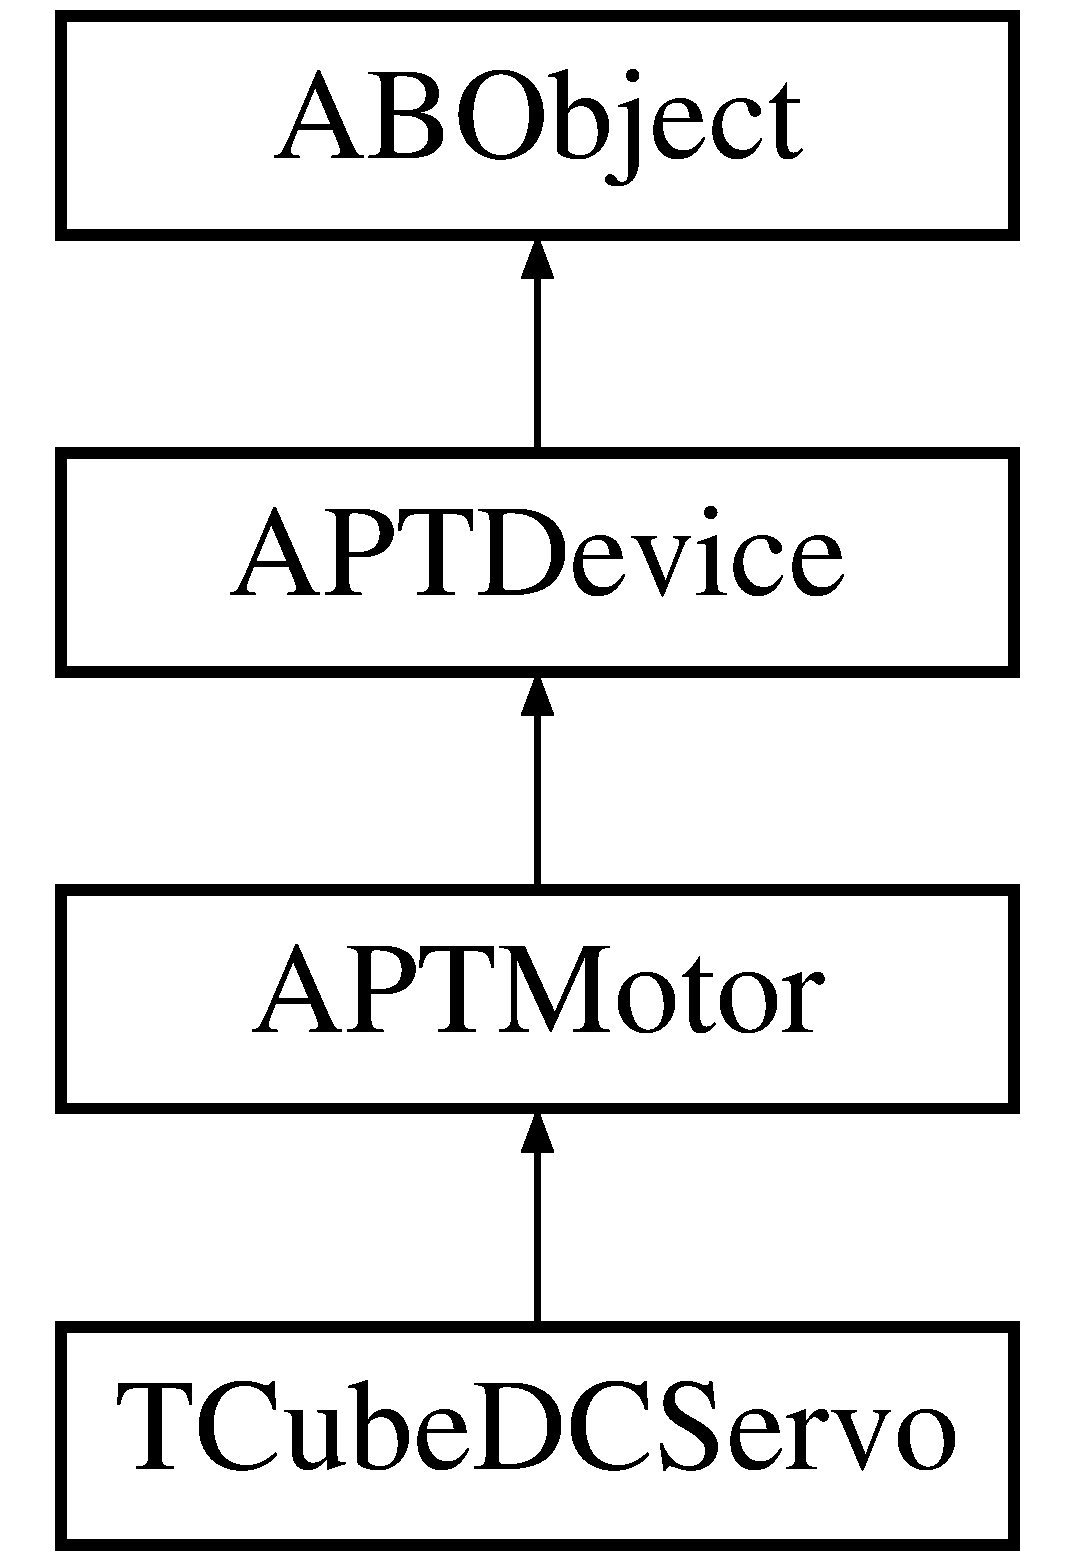
\includegraphics[height=4.000000cm]{class_a_p_t_device}
\end{center}
\end{figure}
\subsection*{Public Member Functions}
\begin{DoxyCompactItemize}
\item 
{\bfseries A\+P\+T\+Device} (int serial)\hypertarget{class_a_p_t_device_a689fd8cfcf7b00be3c3978977841ad16}{}\label{class_a_p_t_device_a689fd8cfcf7b00be3c3978977841ad16}

\item 
bool {\bfseries is\+Connected} ()\hypertarget{class_a_p_t_device_af79731bcc9de5e8c6cb4554c9c5ab728}{}\label{class_a_p_t_device_af79731bcc9de5e8c6cb4554c9c5ab728}

\item 
virtual bool {\bfseries connect} ()=0\hypertarget{class_a_p_t_device_a35a91d8e1989b65fafa10e4006b3efbb}{}\label{class_a_p_t_device_a35a91d8e1989b65fafa10e4006b3efbb}

\item 
virtual bool {\bfseries disconnect} ()=0\hypertarget{class_a_p_t_device_a538be58319f62fcb91bda97a16ce5850}{}\label{class_a_p_t_device_a538be58319f62fcb91bda97a16ce5850}

\item 
virtual bool {\bfseries identify} ()=0\hypertarget{class_a_p_t_device_a1f340e1712035518e60f0087c52c1ff0}{}\label{class_a_p_t_device_a1f340e1712035518e60f0087c52c1ff0}

\item 
bool {\bfseries enable} ()\hypertarget{class_a_p_t_device_a52c413688ce7be304ddfc3259c09e659}{}\label{class_a_p_t_device_a52c413688ce7be304ddfc3259c09e659}

\item 
bool {\bfseries disable} ()\hypertarget{class_a_p_t_device_a7b4fbb10d3ed7551b8c3328f654157ab}{}\label{class_a_p_t_device_a7b4fbb10d3ed7551b8c3328f654157ab}

\item 
string {\bfseries get\+Serial} ()\hypertarget{class_a_p_t_device_ad82cad5cb10407cde9940d634ae9d195}{}\label{class_a_p_t_device_ad82cad5cb10407cde9940d634ae9d195}

\end{DoxyCompactItemize}
\subsection*{Protected Attributes}
\begin{DoxyCompactItemize}
\item 
string {\bfseries m\+Serial}\hypertarget{class_a_p_t_device_a84777e2ac99df354edcbbccf881df188}{}\label{class_a_p_t_device_a84777e2ac99df354edcbbccf881df188}

\item 
Properties {\bfseries m\+Settings}\hypertarget{class_a_p_t_device_ae2712ffda64d717fe01e4433f119024c}{}\label{class_a_p_t_device_ae2712ffda64d717fe01e4433f119024c}

\item 
Device\+Type\+ID {\bfseries m\+Device\+Type\+ID}\hypertarget{class_a_p_t_device_ae326c547996edf6c317fedf922eafd32}{}\label{class_a_p_t_device_ae326c547996edf6c317fedf922eafd32}

\item 
bool {\bfseries m\+Is\+Connected}\hypertarget{class_a_p_t_device_adf44aaf78a088e71a5eadd3854be193f}{}\label{class_a_p_t_device_adf44aaf78a088e71a5eadd3854be193f}

\item 
bool {\bfseries m\+Is\+Active}\hypertarget{class_a_p_t_device_a5cbf066ccd0c6ec7207f4e288b7ac80d}{}\label{class_a_p_t_device_a5cbf066ccd0c6ec7207f4e288b7ac80d}

\end{DoxyCompactItemize}


\subsection{Detailed Description}


Definition at line 11 of file ab\+A\+P\+T\+Device.\+h.



The documentation for this class was generated from the following files\+:\begin{DoxyCompactItemize}
\item 
source/ab\+A\+P\+T\+Device.\+h\item 
source/ab\+A\+P\+T\+Device.\+cpp\end{DoxyCompactItemize}

\hypertarget{class_a_p_t_motor}{}\section{A\+P\+T\+Motor Class Reference}
\label{class_a_p_t_motor}\index{A\+P\+T\+Motor@{A\+P\+T\+Motor}}
Inheritance diagram for A\+P\+T\+Motor\+:\begin{figure}[H]
\begin{center}
\leavevmode
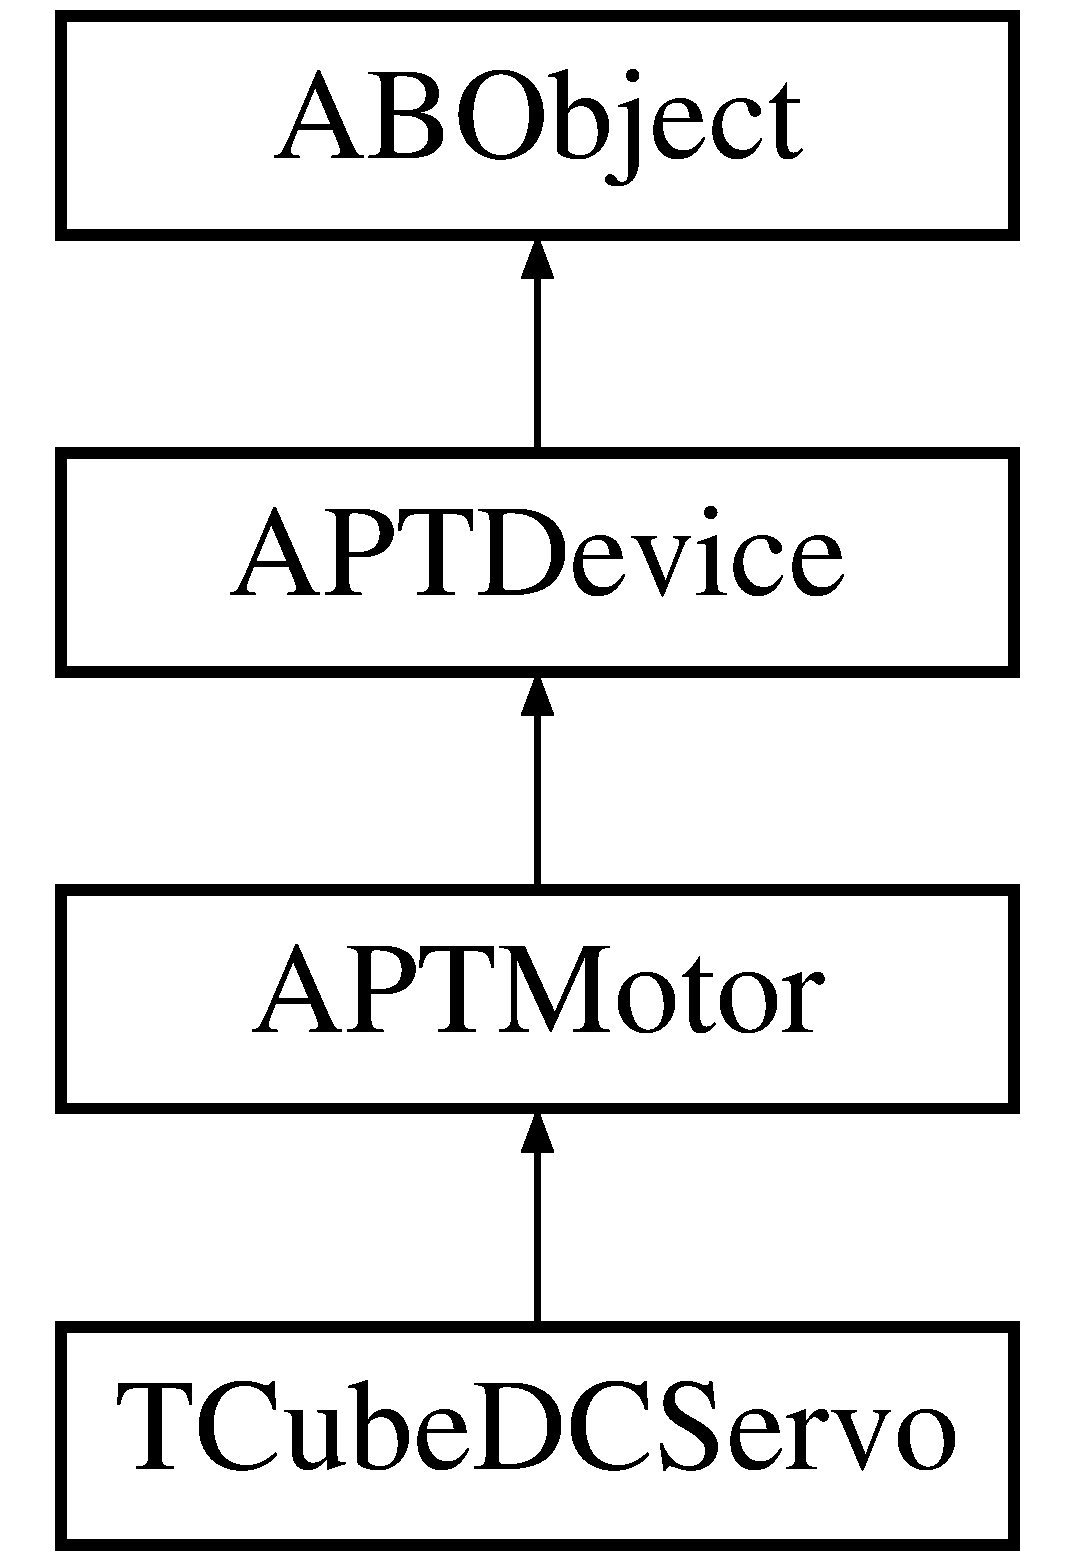
\includegraphics[height=4.000000cm]{class_a_p_t_motor}
\end{center}
\end{figure}
\subsection*{Public Member Functions}
\begin{DoxyCompactItemize}
\item 
{\bfseries A\+P\+T\+Motor} (int serial)\hypertarget{class_a_p_t_motor_a05a9fe8575fe7bfaf73d285704989827}{}\label{class_a_p_t_motor_a05a9fe8575fe7bfaf73d285704989827}

\item 
virtual bool {\bfseries is\+Active} ()=0\hypertarget{class_a_p_t_motor_a7796d2ed550cb3642a9a97e2f99f781c}{}\label{class_a_p_t_motor_a7796d2ed550cb3642a9a97e2f99f781c}

\item 
virtual bool {\bfseries is\+Homed} ()=0\hypertarget{class_a_p_t_motor_afb1d3d08eb946872d65d78d3c40afc04}{}\label{class_a_p_t_motor_afb1d3d08eb946872d65d78d3c40afc04}

\item 
virtual bool {\bfseries is\+Homing} ()=0\hypertarget{class_a_p_t_motor_aa85ccf20174e8c15d3eb5e20e7811e1c}{}\label{class_a_p_t_motor_aa85ccf20174e8c15d3eb5e20e7811e1c}

\item 
virtual bool {\bfseries connect} ()=0\hypertarget{class_a_p_t_motor_a283bc93f03eb9a54ebfab749444cb739}{}\label{class_a_p_t_motor_a283bc93f03eb9a54ebfab749444cb739}

\item 
virtual bool {\bfseries disconnect} ()=0\hypertarget{class_a_p_t_motor_a5370e0fdf73cf0e241f493ab5d4418b9}{}\label{class_a_p_t_motor_a5370e0fdf73cf0e241f493ab5d4418b9}

\item 
virtual bool {\bfseries start\+Polling} ()=0\hypertarget{class_a_p_t_motor_a61ced435fd126a5d04566d76265ad6aa}{}\label{class_a_p_t_motor_a61ced435fd126a5d04566d76265ad6aa}

\item 
virtual bool {\bfseries stop\+Polling} ()=0\hypertarget{class_a_p_t_motor_a87ac54bf651f4bb21edb754326f07221}{}\label{class_a_p_t_motor_a87ac54bf651f4bb21edb754326f07221}

\item 
virtual long \hyperlink{class_a_p_t_motor_ac2ebfd02659a1b1ef8847f99ce7db9ee}{get\+Position} ()=0\hypertarget{class_a_p_t_motor_ac2ebfd02659a1b1ef8847f99ce7db9ee}{}\label{class_a_p_t_motor_ac2ebfd02659a1b1ef8847f99ce7db9ee}

\begin{DoxyCompactList}\small\item\em General commands. \end{DoxyCompactList}\item 
virtual double {\bfseries get\+Velocity} ()=0\hypertarget{class_a_p_t_motor_aabe9fbb03e1ccd51990969beb46ed242}{}\label{class_a_p_t_motor_aabe9fbb03e1ccd51990969beb46ed242}

\item 
virtual double {\bfseries get\+Acceleration} ()=0\hypertarget{class_a_p_t_motor_a74b061f1f03449e112d9b03138427020}{}\label{class_a_p_t_motor_a74b061f1f03449e112d9b03138427020}

\item 
virtual unsigned long {\bfseries get\+Status\+Bits} ()=0\hypertarget{class_a_p_t_motor_a154652d2161514547d9f928ca7ecae3e}{}\label{class_a_p_t_motor_a154652d2161514547d9f928ca7ecae3e}

\item 
virtual void \hyperlink{class_a_p_t_motor_a6b9fd63180ace89c56f4fcd56d4ddfa9}{home} ()=0\hypertarget{class_a_p_t_motor_a6b9fd63180ace89c56f4fcd56d4ddfa9}{}\label{class_a_p_t_motor_a6b9fd63180ace89c56f4fcd56d4ddfa9}

\begin{DoxyCompactList}\small\item\em Control commands. \end{DoxyCompactList}\item 
virtual void {\bfseries stop} ()=0\hypertarget{class_a_p_t_motor_a63cfe446c355e949b82d506fcf85cf70}{}\label{class_a_p_t_motor_a63cfe446c355e949b82d506fcf85cf70}

\item 
virtual void {\bfseries jog\+Forward} ()=0\hypertarget{class_a_p_t_motor_a0bb4d20c8dd6031699239b9f900fdb6f}{}\label{class_a_p_t_motor_a0bb4d20c8dd6031699239b9f900fdb6f}

\item 
virtual void {\bfseries jog\+Backward} ()=0\hypertarget{class_a_p_t_motor_ac6daef63ef5eb26b29b7b4df2a4a6dc0}{}\label{class_a_p_t_motor_ac6daef63ef5eb26b29b7b4df2a4a6dc0}

\item 
virtual void {\bfseries move\+Forward} ()=0\hypertarget{class_a_p_t_motor_adb39b12c71458a8865118123d27026ab}{}\label{class_a_p_t_motor_adb39b12c71458a8865118123d27026ab}

\item 
virtual void {\bfseries move\+Backward} ()=0\hypertarget{class_a_p_t_motor_a4fe7c7dc47f1d4378781b0f338caa914}{}\label{class_a_p_t_motor_a4fe7c7dc47f1d4378781b0f338caa914}

\item 
virtual void {\bfseries move\+Distance} (double distance)=0\hypertarget{class_a_p_t_motor_a109ecfbfb34bca32fa7a453f702ebd59}{}\label{class_a_p_t_motor_a109ecfbfb34bca32fa7a453f702ebd59}

\item 
virtual bool {\bfseries identify} ()=0\hypertarget{class_a_p_t_motor_a39036449d88ca4ea1774228aee4c4eb6}{}\label{class_a_p_t_motor_a39036449d88ca4ea1774228aee4c4eb6}

\end{DoxyCompactItemize}
\subsection*{Protected Attributes}
\begin{DoxyCompactItemize}
\item 
Timer {\bfseries m\+Status\+Timer}\hypertarget{class_a_p_t_motor_aab58a6e523dc74f486fd1c45869dad33}{}\label{class_a_p_t_motor_aab58a6e523dc74f486fd1c45869dad33}

\item 
unsigned long {\bfseries m\+Status\+Bits}\hypertarget{class_a_p_t_motor_ad3f322af6da98d4193f0c0b3f1b55471}{}\label{class_a_p_t_motor_ad3f322af6da98d4193f0c0b3f1b55471}

\item 
\hyperlink{struct_scaling_factors}{Scaling\+Factors} {\bfseries m\+Scaling\+Factors}\hypertarget{class_a_p_t_motor_ac7dc5734487a985f1522b57ffd2da8f8}{}\label{class_a_p_t_motor_ac7dc5734487a985f1522b57ffd2da8f8}

\end{DoxyCompactItemize}


\subsection{Detailed Description}


Definition at line 16 of file ab\+A\+P\+T\+Motor.\+h.



The documentation for this class was generated from the following files\+:\begin{DoxyCompactItemize}
\item 
source/ab\+A\+P\+T\+Motor.\+h\item 
source/ab\+A\+P\+T\+Motor.\+cpp\end{DoxyCompactItemize}

\hypertarget{class_device_manager}{}\section{Device\+Manager Class Reference}
\label{class_device_manager}\index{Device\+Manager@{Device\+Manager}}
Inheritance diagram for Device\+Manager\+:\begin{figure}[H]
\begin{center}
\leavevmode
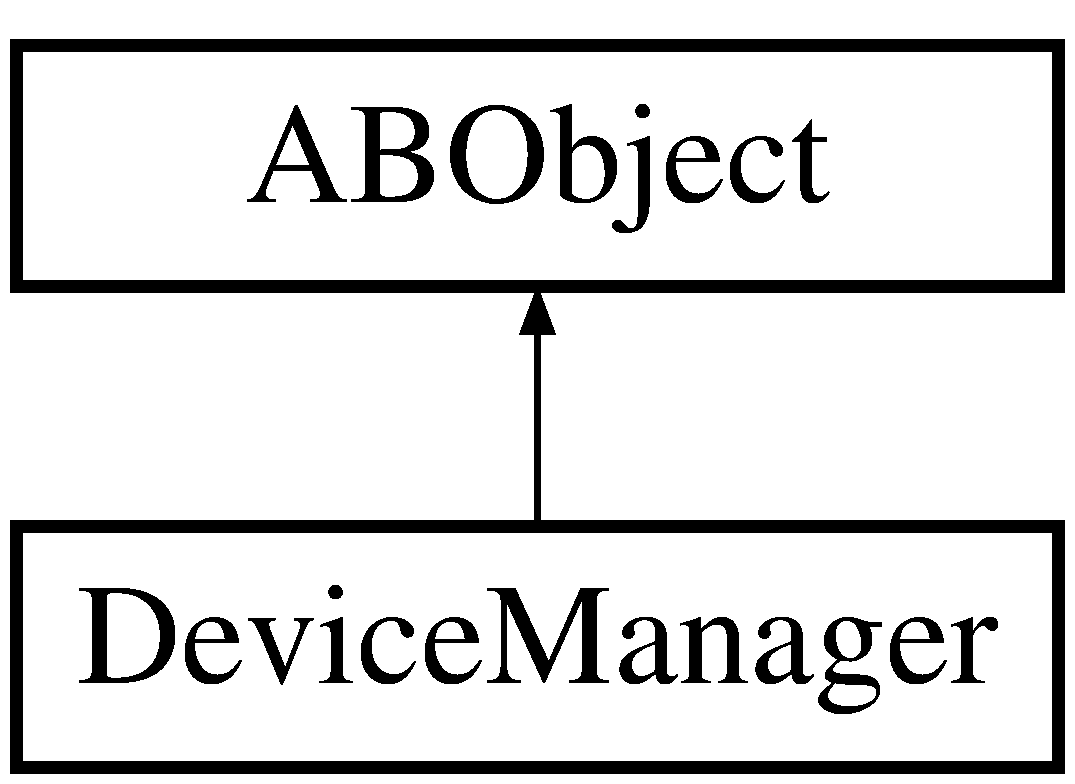
\includegraphics[height=2.000000cm]{class_device_manager}
\end{center}
\end{figure}
\subsection*{Public Member Functions}
\begin{DoxyCompactItemize}
\item 
\hyperlink{class_a_p_t_device}{A\+P\+T\+Device} $\ast$ {\bfseries connect\+Device} (int serial)\hypertarget{class_device_manager_ac0ce1a37822574594eb65f02465d2c00}{}\label{class_device_manager_ac0ce1a37822574594eb65f02465d2c00}

\item 
int {\bfseries connect\+All\+Devices} ()\hypertarget{class_device_manager_a44bad7c44e967d498b4aa44d2d99ba61}{}\label{class_device_manager_a44bad7c44e967d498b4aa44d2d99ba61}

\item 
bool {\bfseries dis\+Connect} (\hyperlink{class_a_p_t_device}{A\+P\+T\+Device} $\ast$device=N\+U\+LL)\hypertarget{class_device_manager_aae705d733108941034673f80669d05b8}{}\label{class_device_manager_aae705d733108941034673f80669d05b8}

\item 
bool {\bfseries dis\+Connect\+All} ()\hypertarget{class_device_manager_a6cdff3988b15f8ccfa857c723ea94d31}{}\label{class_device_manager_a6cdff3988b15f8ccfa857c723ea94d31}

\item 
string {\bfseries get\+Info} () const \hypertarget{class_device_manager_ad614cb5000d81785ae831b27aaa6d887}{}\label{class_device_manager_ad614cb5000d81785ae831b27aaa6d887}

\item 
String\+List {\bfseries get\+Device\+Serials} () const \hypertarget{class_device_manager_ad8757315554fabd3f1dcb852be6094a6}{}\label{class_device_manager_ad8757315554fabd3f1dcb852be6094a6}

\item 
int {\bfseries get\+Number\+Of\+Connectable\+Devices} () const \hypertarget{class_device_manager_a41df406e20602c881d1c1cd2c80bdb4e}{}\label{class_device_manager_a41df406e20602c881d1c1cd2c80bdb4e}

\item 
int {\bfseries get\+Number\+Of\+Connected\+Devices} () const \hypertarget{class_device_manager_aa1504b362aaac787513d2b2bfabcaa86}{}\label{class_device_manager_aa1504b362aaac787513d2b2bfabcaa86}

\item 
\hyperlink{class_a_p_t_device}{A\+P\+T\+Device} $\ast$ {\bfseries get\+Device} (int serial)\hypertarget{class_device_manager_a6afa6667cca657ed2527a9e3c46df3d3}{}\label{class_device_manager_a6afa6667cca657ed2527a9e3c46df3d3}

\item 
\hyperlink{class_a_p_t_device}{A\+P\+T\+Device} $\ast$ {\bfseries get\+First} () const \hypertarget{class_device_manager_a87d4bd700cd87b0b5b0e9a974536137f}{}\label{class_device_manager_a87d4bd700cd87b0b5b0e9a974536137f}

\item 
\hyperlink{class_a_p_t_device}{A\+P\+T\+Device} $\ast$ {\bfseries get\+Next} () const \hypertarget{class_device_manager_aa8a9e2b99c7ba69d85786b1be5f899c0}{}\label{class_device_manager_aa8a9e2b99c7ba69d85786b1be5f899c0}

\item 
\hyperlink{class_a_p_t_device}{A\+P\+T\+Device} $\ast$ {\bfseries get\+Previous} () const \hypertarget{class_device_manager_a9abe7a53a853fcc620ebd489d685a17d}{}\label{class_device_manager_a9abe7a53a853fcc620ebd489d685a17d}

\item 
\hyperlink{class_a_p_t_device}{A\+P\+T\+Device} $\ast$ {\bfseries get\+Current} () const \hypertarget{class_device_manager_ac1738a2162299622e41764bef8ee7bd7}{}\label{class_device_manager_ac1738a2162299622e41764bef8ee7bd7}

\end{DoxyCompactItemize}
\subsection*{Friends}
\begin{DoxyCompactItemize}
\item 
A\+B\+\_\+\+C\+O\+RE friend ostream \& {\bfseries operator$<$$<$} (ostream \&os, \hyperlink{class_device_manager}{Device\+Manager} \&pm)\hypertarget{class_device_manager_aeac7252d4c4a31b9b427e75bd730b59a}{}\label{class_device_manager_aeac7252d4c4a31b9b427e75bd730b59a}

\end{DoxyCompactItemize}


\subsection{Detailed Description}


Definition at line 20 of file ab\+Device\+Manager.\+h.



The documentation for this class was generated from the following files\+:\begin{DoxyCompactItemize}
\item 
source/ab\+Device\+Manager.\+h\item 
source/ab\+Device\+Manager.\+cpp\end{DoxyCompactItemize}

\hypertarget{struct_scaling_factors}{}\section{Scaling\+Factors Struct Reference}
\label{struct_scaling_factors}\index{Scaling\+Factors@{Scaling\+Factors}}


{\ttfamily \#include $<$ab\+A\+P\+T\+Motor.\+h$>$}

\subsection*{Public Attributes}
\begin{DoxyCompactItemize}
\item 
double {\bfseries position}\hypertarget{struct_scaling_factors_ad44893e5393c09251d1988ce6a710a21}{}\label{struct_scaling_factors_ad44893e5393c09251d1988ce6a710a21}

\item 
double {\bfseries velocity}\hypertarget{struct_scaling_factors_ac036c7d85dc520a41e56e9275a261d12}{}\label{struct_scaling_factors_ac036c7d85dc520a41e56e9275a261d12}

\item 
double {\bfseries acceleration}\hypertarget{struct_scaling_factors_a54b1f17a7fba729deba581e36db6cb64}{}\label{struct_scaling_factors_a54b1f17a7fba729deba581e36db6cb64}

\end{DoxyCompactItemize}


\subsection{Detailed Description}
Scaling factors are used to convert a motors position, velocity and accelertation expressed in device units, into world physical units. 

Definition at line 9 of file ab\+A\+P\+T\+Motor.\+h.



The documentation for this struct was generated from the following file\+:\begin{DoxyCompactItemize}
\item 
source/ab\+A\+P\+T\+Motor.\+h\end{DoxyCompactItemize}

\hypertarget{class_t_cube_d_c_servo}{}\section{T\+Cube\+D\+C\+Servo Class Reference}
\label{class_t_cube_d_c_servo}\index{T\+Cube\+D\+C\+Servo@{T\+Cube\+D\+C\+Servo}}
Inheritance diagram for T\+Cube\+D\+C\+Servo\+:\begin{figure}[H]
\begin{center}
\leavevmode
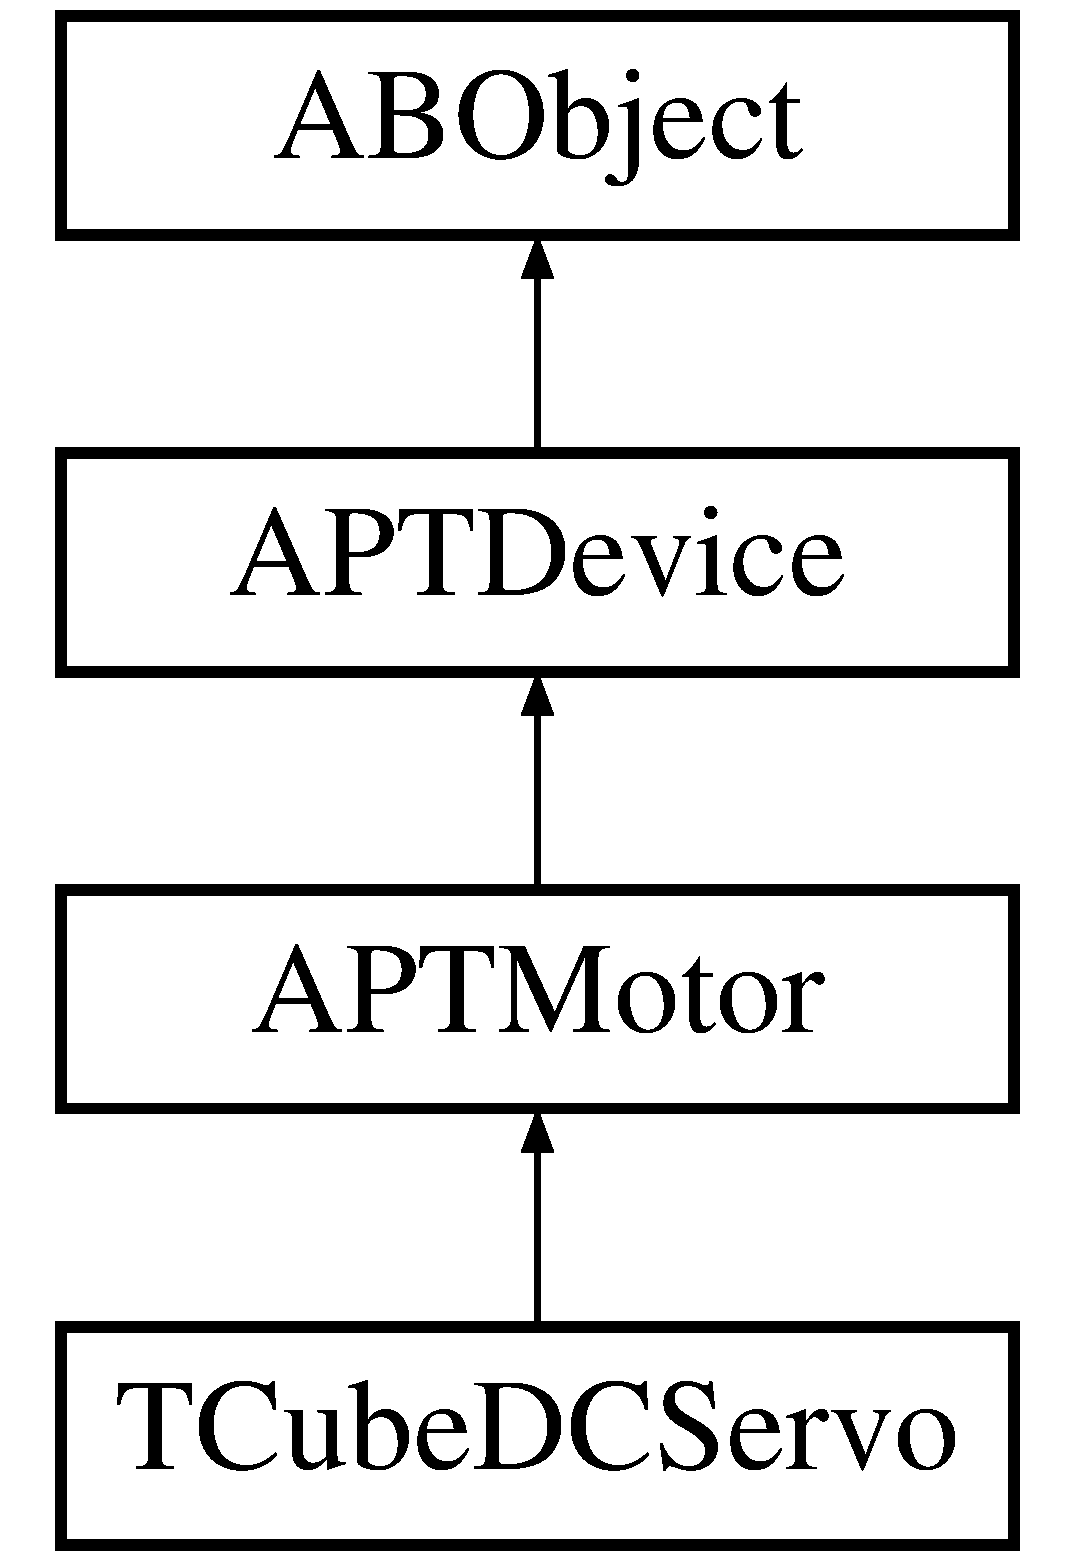
\includegraphics[height=4.000000cm]{class_t_cube_d_c_servo}
\end{center}
\end{figure}
\subsection*{Public Member Functions}
\begin{DoxyCompactItemize}
\item 
{\bfseries T\+Cube\+D\+C\+Servo} (int serial)\hypertarget{class_t_cube_d_c_servo_a31ea7bdfce103f01dbc82e7ec3abede7}{}\label{class_t_cube_d_c_servo_a31ea7bdfce103f01dbc82e7ec3abede7}

\item 
bool \hyperlink{class_t_cube_d_c_servo_a756f667bda8e714d7e3e2fd19f84ff42}{is\+Active} ()\hypertarget{class_t_cube_d_c_servo_a756f667bda8e714d7e3e2fd19f84ff42}{}\label{class_t_cube_d_c_servo_a756f667bda8e714d7e3e2fd19f84ff42}

\begin{DoxyCompactList}\small\item\em is\+Active checks if the device is active. \end{DoxyCompactList}\item 
bool {\bfseries is\+Homing} ()\hypertarget{class_t_cube_d_c_servo_a4d85d3523736a4013d2f727313426f68}{}\label{class_t_cube_d_c_servo_a4d85d3523736a4013d2f727313426f68}

\item 
bool {\bfseries is\+Homed} ()\hypertarget{class_t_cube_d_c_servo_a2e56f6537586a0050c6b6edb745a627e}{}\label{class_t_cube_d_c_servo_a2e56f6537586a0050c6b6edb745a627e}

\item 
bool {\bfseries connect} ()\hypertarget{class_t_cube_d_c_servo_afb574051761c7704d30f5d4601f7a87f}{}\label{class_t_cube_d_c_servo_afb574051761c7704d30f5d4601f7a87f}

\item 
bool {\bfseries disconnect} ()\hypertarget{class_t_cube_d_c_servo_a5c6947759798bcf4ddde5e6184f947ab}{}\label{class_t_cube_d_c_servo_a5c6947759798bcf4ddde5e6184f947ab}

\item 
bool {\bfseries start\+Polling} ()\hypertarget{class_t_cube_d_c_servo_acae5a43c5ec4741da9c71a23135177c3}{}\label{class_t_cube_d_c_servo_acae5a43c5ec4741da9c71a23135177c3}

\item 
bool {\bfseries stop\+Polling} ()\hypertarget{class_t_cube_d_c_servo_aa3e0f3ada53bbb08aae20b71e54ae33a}{}\label{class_t_cube_d_c_servo_aa3e0f3ada53bbb08aae20b71e54ae33a}

\item 
long \hyperlink{class_t_cube_d_c_servo_a0786a6f3dea544aea859fddbfbe1a8c4}{get\+Position} ()\hypertarget{class_t_cube_d_c_servo_a0786a6f3dea544aea859fddbfbe1a8c4}{}\label{class_t_cube_d_c_servo_a0786a6f3dea544aea859fddbfbe1a8c4}

\begin{DoxyCompactList}\small\item\em General commands. \end{DoxyCompactList}\item 
double {\bfseries get\+Velocity} ()\hypertarget{class_t_cube_d_c_servo_a5f7c1fbbb0f039250877f7f027cb9c4c}{}\label{class_t_cube_d_c_servo_a5f7c1fbbb0f039250877f7f027cb9c4c}

\item 
double {\bfseries get\+Acceleration} ()\hypertarget{class_t_cube_d_c_servo_aa1ad26df8337681f5916dd486273e594}{}\label{class_t_cube_d_c_servo_aa1ad26df8337681f5916dd486273e594}

\item 
unsigned long {\bfseries get\+Status\+Bits} ()\hypertarget{class_t_cube_d_c_servo_ae204b5c21b4caff2945a15d532656257}{}\label{class_t_cube_d_c_servo_ae204b5c21b4caff2945a15d532656257}

\item 
void \hyperlink{class_t_cube_d_c_servo_a6921245c24f8f0c2c9416ec31a5ed79b}{home} ()\hypertarget{class_t_cube_d_c_servo_a6921245c24f8f0c2c9416ec31a5ed79b}{}\label{class_t_cube_d_c_servo_a6921245c24f8f0c2c9416ec31a5ed79b}

\begin{DoxyCompactList}\small\item\em Control commands. \end{DoxyCompactList}\item 
void {\bfseries stop} ()\hypertarget{class_t_cube_d_c_servo_a56df33090fa949a9b94cab3779e69026}{}\label{class_t_cube_d_c_servo_a56df33090fa949a9b94cab3779e69026}

\item 
void {\bfseries jog\+Forward} ()\hypertarget{class_t_cube_d_c_servo_a6102f5d529f1122f5e9ebac31e5df0f4}{}\label{class_t_cube_d_c_servo_a6102f5d529f1122f5e9ebac31e5df0f4}

\item 
void {\bfseries jog\+Backward} ()\hypertarget{class_t_cube_d_c_servo_a1aa493050ddf55d7363e03a0edc15fa6}{}\label{class_t_cube_d_c_servo_a1aa493050ddf55d7363e03a0edc15fa6}

\item 
void {\bfseries move\+Forward} ()\hypertarget{class_t_cube_d_c_servo_aaff34acc572b7c385c7d761fb9d17b4c}{}\label{class_t_cube_d_c_servo_aaff34acc572b7c385c7d761fb9d17b4c}

\item 
void {\bfseries move\+Backward} ()\hypertarget{class_t_cube_d_c_servo_a2339bc46a8c2434273157a721933a4b1}{}\label{class_t_cube_d_c_servo_a2339bc46a8c2434273157a721933a4b1}

\item 
void {\bfseries move\+Distance} (double distance)\hypertarget{class_t_cube_d_c_servo_a5fbed128911d93cd01f461ea3e031d90}{}\label{class_t_cube_d_c_servo_a5fbed128911d93cd01f461ea3e031d90}

\item 
bool {\bfseries identify} ()\hypertarget{class_t_cube_d_c_servo_aa8513d736e0e795921c0d4d85783ba53}{}\label{class_t_cube_d_c_servo_aa8513d736e0e795921c0d4d85783ba53}

\end{DoxyCompactItemize}
\subsection*{Additional Inherited Members}


\subsection{Detailed Description}


Definition at line 6 of file ab\+T\+Cube\+D\+C\+Servo.\+h.



The documentation for this class was generated from the following files\+:\begin{DoxyCompactItemize}
\item 
source/ab\+T\+Cube\+D\+C\+Servo.\+h\item 
source/ab\+T\+Cube\+D\+C\+Servo.\+cpp\end{DoxyCompactItemize}

\hypertarget{class_thor_labs_data}{}\section{Thor\+Labs\+Data Class Reference}
\label{class_thor_labs_data}\index{Thor\+Labs\+Data@{Thor\+Labs\+Data}}
\subsection*{Public Member Functions}
\begin{DoxyCompactItemize}
\item 
string {\bfseries get\+Device\+Type\+Name} (int id)\hypertarget{class_thor_labs_data_a88fe2eb9ffdafbc7779a665fd0231a80}{}\label{class_thor_labs_data_a88fe2eb9ffdafbc7779a665fd0231a80}

\end{DoxyCompactItemize}


\subsection{Detailed Description}


Definition at line 14 of file ab\+T\+L\+Wrapper.\+h.



The documentation for this class was generated from the following files\+:\begin{DoxyCompactItemize}
\item 
source/ab\+T\+L\+Wrapper.\+h\item 
source/ab\+T\+L\+Wrapper.\+cpp\end{DoxyCompactItemize}

%--- End generated contents ---

% Index
\backmatter
\newpage
\phantomsection
\clearemptydoublepage
\addcontentsline{toc}{chapter}{Index}
\printindex

\end{document}
